\chapter{Methodology}
\label{Methodology}

In this section we introduce the methodology for our proposed method for the task of human pose estimation using point cloud. As we reviewed in \ref{Related work} the key issue of any which use point clouds as an input is huge spatial variation of the data. Point clouds much diverse compared to 2D images in terms of location and rotation. Capsule networks shows promising results \parencite{sabour_dynamic_2017} on 2D data, and better handle spatial invariance compared to regular NN models.  \\
The chapter consists of two main section. In \ref{Data preparation} section we will cover the preprocessing for the input data and ground truths, and methods of adding artificial noise the the input data. In \ref{Network architecture} we will cover the network's architecture and algorithms for performing network's training.


\section{Data preparation}
\label{Data preparation}
In this section we will cover main preprocessing steps for datasets. Preprocessing consists of:
\begin{enumerate}
  \item human extraction;
  \begin{enumerate}
    \item threshold filtering;
    \item clusterization \& cluster selection;
  \end{enumerate}
  \item point cloud normalization;
  \item adding noise to data (optional).
\end{enumerate}

On the first step we remove the most obvious points which doesn't represent human posture. On the second step we perform segmentation to extract "human" cluster. The third step is optional, and is used in experiments with performance of different models with various levels of the noise.


\subsection{Human extraction}
To start working with points cloud for human pose estimation we decided to extract human human points out of overall point cloud. As we can see from the Figure \ref{img:example-of-raw-data}, the raw point cloud contains not only human point cloud but also other objects which are located in the room, such as walls, cupboards, and other objects. These obstacles will not only harm the model's performance but will also greatly slow down the model's training and inference due to excess number of point.

\begin{figure}[htbp]
    \centerline{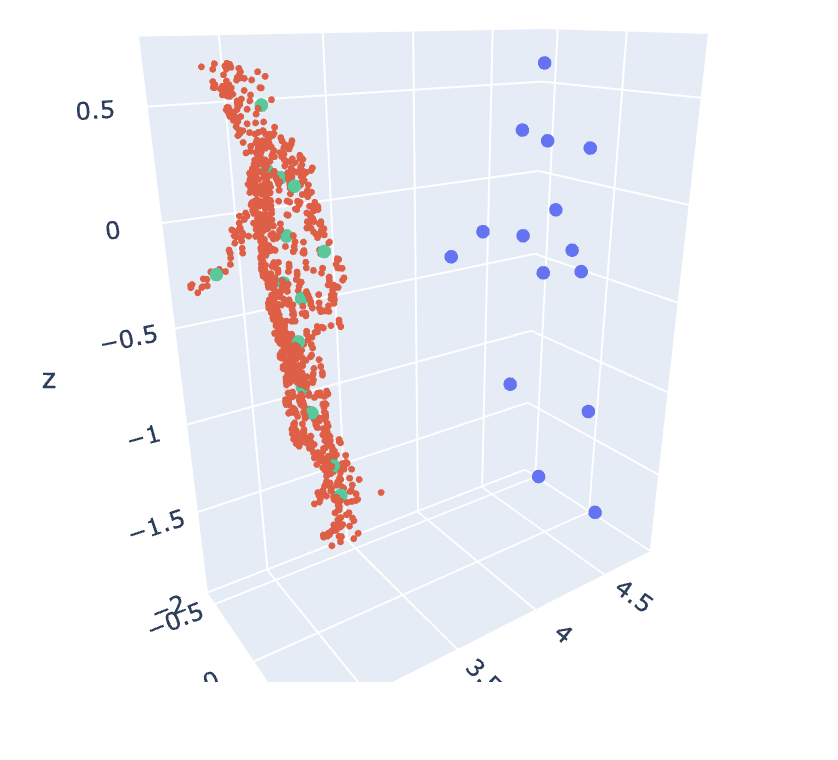
\includegraphics[scale=.4]{Figures/template.png}}
    \caption{Example of raw data from ITOP dataset (front view)}
    \label{img:example-of-raw-data}
\end{figure}

\subsubsection{Threshold filtering}
\label{s:threshold-filtering}
Threshold filtering is the first step in preprocessing pipeline. The aim of this step is to filter out the most obvious points which don't belong to the human posture.
After manual checks we came up to such parameters:  

\begin{equation}
    \begin{aligned}
        x_{min} &= -1   &x_{max} &= 1 \\
        y_{min} &= -1.4 &y_{max} &= 2 \\
        z_{min} &= -1.5 &z_{max} &= 3.5
    \end{aligned}
\label{eqn:threshold-values}
\end{equation}

\ref{eqn:threshold-values} sets min-max distance values from camera view. The camera sensor is considered as center - $(0, 0, 0)$. In this way, $x$ coordinate represents left-right direction from the camera center, $y$ - top-bottom, and $z$ - the depth. \\
An example of threshold filtered point cloud could be seen in Figure~\ref{img:after-threshold-filtering}.

\begin{figure}[htbp]
    \centerline{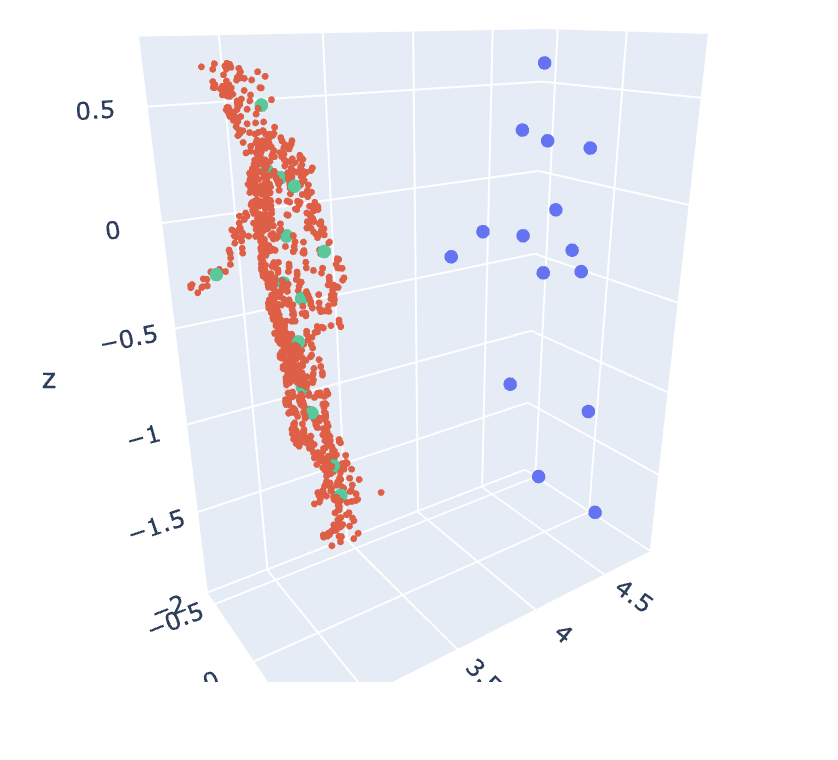
\includegraphics[scale=.4]{Figures/template.png}}
    \caption{Example of point cloud after applying of threshold filter}
    \label{img:after-threshold-filtering}
\end{figure}

\subsubsection{Clusterization}
The next step in preprocessing is clusterization \& extraction. On this step we clusterize point cloud from the \ref{s:threshold-filtering} and extract the human cluster. For clusterization step we propose the nearest-neighbour search algorithm \parencite{noauthor_nearest_2021} with kd-tree data-structure, using FLANN \footnote{Fast Library for Approximate Nearest Neighbor}. \\
The aim of the clusterization is separate human cluster and small noisy clusters from the point cloud. As we can see from the Algorithm~\ref{alg:clusterization}, for each point in initial point cloud $P$ we try to put it to some cluster based on the distance (radius - $r$) of that cluster. If the distance is less that radius to each cluster then this point creates a new cluster. At the end of clusterization we get a set of clusters $C$. \\
Since the human cluster always the biggest, at the end of clusterization we take the argmax and get human cluster $C_{human}$.

On the Figure~\ref{img:after-clustering} we can see the point cloud before clusterization, after, and the resulting human cluster (the biggest cluster). \\

\begin{algorithm}[H]
\label{alg:clusterization}
\SetAlgoLined
\KwResult{human point cloud cluster - $C_{human}$}
 create a Kd-tree representation for the input point cloud dataset $P$ \;
 set up an empty list of clusters $C$, and a queue of the points that need to be checked $Q$ \;
\For{\texttt{every point} $p_i \in P$} {
    add $p_i$ to the current queue $Q$ \;
    \For{\texttt{every point} $p_i \in Q$}{
        search for the set $P^k_i$ of point neighbors of $p_i$ in a sphere with radius $r < d_{th}$ \;
        for every neighbor $p^k_i \in P^k_i$, check if the point has already been processed, and if not add it to $Q$\;
    }
    when the list of all points in $Q$ has been processed, add $Q$ to the list of clusters $C$, and reset $Q$ to an empty list \;
}
the algorithm terminates when all points $\boldsymbol{p}_i \in P$ have been processed and are now part of the list of point clusters $C$ \;
$C_{human} = \underset{ x \in C }{\arg\max}$

\caption{Point cloud clusterization and human extraction \parencite{noauthor_pcl_nodate}}
\end{algorithm}

\begin{figure}[htbp]
    \centerline{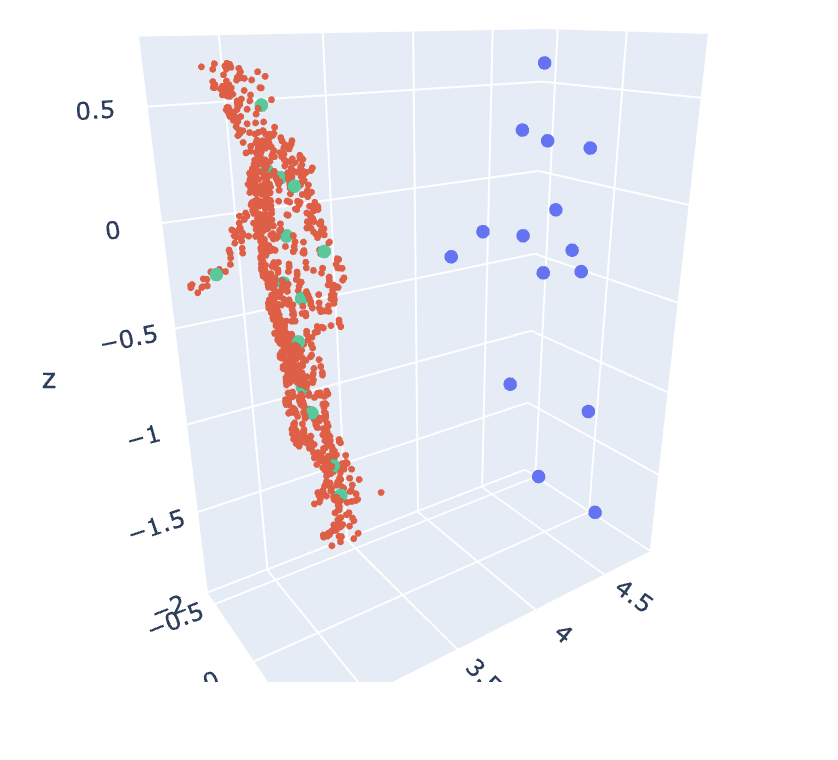
\includegraphics[scale=.4]{Figures/template.png}}
    \caption{Example of point cloud after applying of threshold filter}
    \label{img:after-clustering}
\end{figure}

\subsection{Point cloud normalization}
TBD



\subsection{Adding noise to data}
Noise is the common thing in point cloud data. The origin the the noise could be environment conditions such as dust, fog, and other particles in the air. Also, the noise appears due to unperfectness on the lidar and other tools of creating point clouds.

In Experiment~\ref{s:experiment-noise} we investigate how models perform with different amount of artificial noise in the input data. For that we need to generate the noise which could be similar to the real-world. We propose to use two types of noise:
\begin{itemize}
  \item Gaussian noise;
  \item outlier noise.
\end{itemize}

\subsubsection{Gaussian noise}
The Gaussian noise is adding noise to the initial points in the point cloud $P$. With probability of $p$ the Gaussian noise ($\sigma$, $\mu$) is added to the point $p \in P$. In this way we simulate the unperfectness of the detecting device. The generation process is described in Algorithm~\ref{alg:gaussian-noise}

\begin{algorithm}[H]
\label{alg:gaussian-noise}
\SetAlgoLined
\KwResult{human point cloud with Gaussian noise  - $\hat{P_{human}}$}
\For{\texttt{every point} $p_i \in P$} {
    \If{ \texttt{uniRand()} < $Prob_{noise}$ } {
        Set $p_x$ to $p_x$ + $Gaus(\sigma, \mu)$ \;
        Set $p_y$ to $p_y$ + $Gaus(\sigma, \mu)$ \;
        Set $p_z$ to $p_z$ + $Gaus(\sigma, \mu)$ \;
    }
}
\caption{Adding Gaussian noise to point cloud \parencite{uchida_tom-uchidaadd_noise_to_point_cloud_2021}}
\end{algorithm}

An example of applying the Gaussian noise to the point cloud could be seen in the Figure~\ref{img:gaussian-noise}

\begin{figure}[htbp]
    \centerline{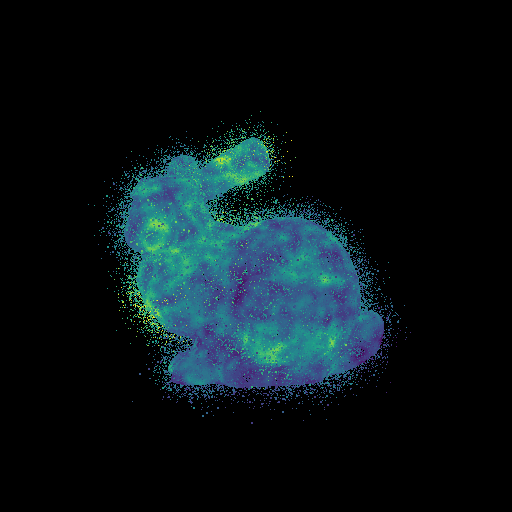
\includegraphics[scale=.6]{Figures/coords_gaussian.png}}
    \caption{Example of pllying the Gaussian noise to the point cloud \parencite{uchida_tom-uchidaadd_noise_to_point_cloud_2021}}
    \label{img:gaussian-noise}
\end{figure}

\subsubsection{Outlier noise}
The outlier noise adding new points to the initial point cloud $P$. The amount of outlier noise is defined by the fraction of the noise points compared to the initial number of human points. The noise point is taken from the uniform distribution $U(a, b)$. Where $a$ and $b$ are min-max values from the initial point cloud. In this way, outlier noise will fill uniformly the bounding box of the initial point cloud.

An example of addition of the outlier noise to the point cloud could be seen in the Figure~\ref{img:outlier-noise}

\begin{figure}[htbp]
    \centerline{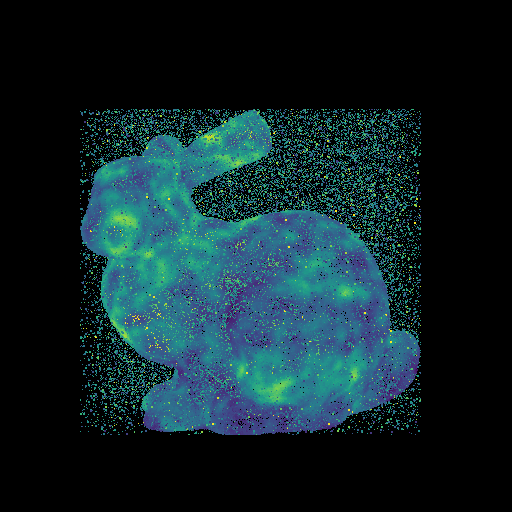
\includegraphics[scale=.6]{Figures/coords_outlier.png}}
    \caption{Example of addition the outlier noise to the point cloud \parencite{uchida_tom-uchidaadd_noise_to_point_cloud_2021}}
    \label{img:outlier-noise}
\end{figure}

\section{Network architecture}
\label{Network architecture}
\subsection{Capsule network autoencoder}
\subsubsection{Chamfer distance}
\subsection{Capsule-based regression network}

\section{Network training}

